\documentclass[mathNotesPreamble]{subfiles}
\begin{document}
%\relscale{1.4} %TODO
\section{16.4: Triple Integrals}



  \begin{thmBox*}[Theorem 16.5: Triple Integrals]
    Let $f$ be continuous over the region
      \[D=\set{(x,y,z): a\leq x\leq b,\ g(x)\leq y\leq h(x),\ G(x,y)\leq z\leq H(x,y)},\]
    where $g$, $h$, $G$, and $H$ are continuous functions. Then $f$ is integrable over $D$ and the triple integral is evaluated as the iterated integral
      \[\iiint\limits_D f(x,y,z)\,dV=\int_a^b \int_{g(x)}^{h(x)} \int_{G(x,y)}^{H(x,y)} f(x,y,z)\,dz\,dy\,dx.\]
  \end{thmBox*}
  \vspace*{\stretch{1}}
  \begin{center}
    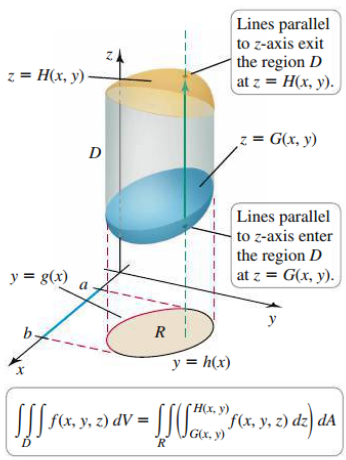
\includegraphics[width=0.29\linewidth, trim={0mm 0.5mm 0mm 0mm},clip]{images/briggs_16_04/fig16_39}
    \hspace*{\stretch{0.5}}
    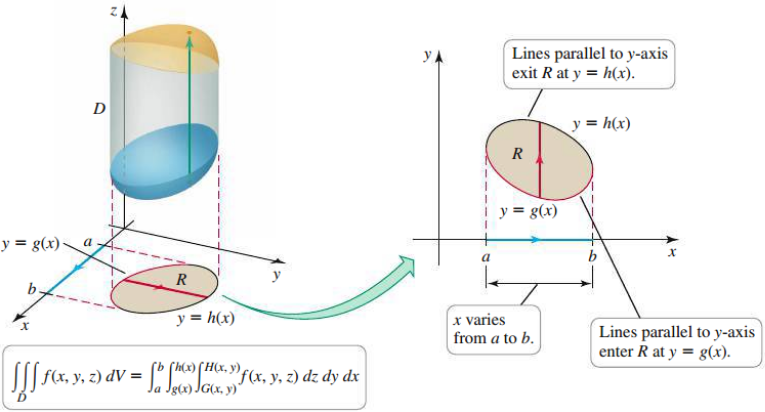
\includegraphics[width=0.68\linewidth]{images/briggs_16_04/fig16_40}
  \end{center}
  \vspace*{\stretch{1}}
  \begin{center}
    \renewcommand{\arraystretch}{1.25}
    \begin{tabular}{@{}lCR@{$\,\leq\,$}C@{$\,\leq\,$}L@{}}\toprule
      \textbf{Integral}& \textbf{Variable}& \multicolumn{3}{c}{\textbf{Interval}}\\
      Inner& z& G(x,y)& z& H(x,y)\\
      Middle& y& g(x)& y& h(x)\\
      Outer& x& a& x& b\\\bottomrule
    \end{tabular}
  \end{center}
  \pagebreak

  \begin{ex*}
    A solid box $D$ is bounded by the planes $x=0$, $x=3$, $y=0$, $y=2$, $z=0$, and $z=1$. The density of the box decreases linearly in the positive $z$-direction and is given by $f(x,y,z)=2-z$. Find the mass of the box.
  \end{ex*}
  \vspace*{\stretch{1}}

  \begin{ex*}
    Find the volume of the prism $D$ in the first octant bounded by the planes $y=4-2x$ and $z=6$.
  \end{ex*}
  \vspace*{\stretch{1}}
  \pagebreak

  \begin{ex*}
    Write the triple integral for $\iiint\limits_D f(x,y,z)\,dV$ where $D$ is a sphere of radius $r$ centered at the origin.
  \end{ex*}
  \vspace*{5\baselineskip}
  \begin{ex*}
    Find the volume of the solid $D$ bounded by the paraboloids $y=x^2+3z^2+1$ and $y=5-3x^2-z^2$.
  \end{ex*}
  \vspace*{\stretch{1}}
  \pagebreak

  \noindent
  The concept of changing the order of integration for double integrals also extends to triple integrals:
  \begin{ex*}
    Consider the integral
      \[\int_0^{\sqrt[4]{\pi}} \int_0^z \int_y^z 12y^2z^3\sin\parens{x^4}\,dx\,dy\,dz.\]
    Sketch the region of integration, then evaluate the integral by changing the order of integration.
  \end{ex*}
  \vspace{\stretch{1}}
  \pagebreak

  \begin{defn*}[Average Value of a Function of Three Variables]
    If $f$ is continuous on a region $D$ of $\bbr^3$, then the \textbf{average value} of $f$ over $D$ is
      \[\bar{f}=\frac{1}{\textnormal{volume of }D}\iiint\limits_D f(x,y,z)\,dV.\]
  \end{defn*}

  \begin{ex*}
    Find the average $y$-coordinate of the points in the standard simplex \newline$D=\set{(x,y,z): x+y+z\leq 1,\, x\geq 0,\, y\geq 0,\, z\geq 0}$.
  \end{ex*}

  \pagebreak
  
\end{document}